\section*{Propagazione del segnale nell'aria}
La propagazione del segnale nell'atmosfera può essere classificata in base alle bande di frequenza e alle relative caratteristiche. Di seguito vengono elencate le diverse bande di classificazione, le iniziali, i range di frequenza e le principali caratteristiche:
\begin{table}[h!]
    \centering
    \begin{tabular}{llll}
        \hline
        \textbf{Classification Band} & \textbf{Initials} & \textbf{Frequency Range} & \textbf{Characteristics} \\
        \hline
        Extremely low frequency      & ELF               & $<$ 300 Hz               & Ground wave              \\
        Very low frequency           & VLF               & 3 kHz - 30 kHz           & Ground/Sky wave          \\
        Low frequency                & LF                & 30 kHz - 300 kHz         & Ground/Sky wave          \\
        Medium frequency             & MF                & 300 kHz - 3 MHz          & Ground/Sky wave          \\
        High frequency               & HF                & 3 MHz - 30 MHz           & Sky wave                 \\
        Very high frequency          & VHF               & 30 MHz - 300 MHz         & Space wave               \\
        Ultra high frequency         & UHF               & 300 MHz - 3 GHz          & Space wave               \\
        Super high frequency         & SHF               & 3 GHz - 30 GHz           & Space wave               \\
        \hline
    \end{tabular}
\end{table}


Dalla frequenza delle onde, da cui dipende la modalità di propagazione attraverso il canale, si identificano i seguenti meccanismi di propagazione:

\begin{itemize}
    \item \textbf{Ground wave} (fino a 2 MHz): le onde si propagano seguendo la curvatura terrestre riuscendo a raggiungere un ricevitore oltre l'orizzonte, in certi casi anche a centinaia di chilometri di distanza, ma i problemi che si pongono sono legati all'utilizzo di una frequenza inferiore a 2 MHz e alla necessità di utilizzare antenne di dimensioni molto grandi. Per esempio sono utilizzate nella sincronizzazione di orologi atomici. Possono essere sfruttate per scopi militari.
    \item \textbf{Sky wave} (3-30 MHz): le onde sono riflesse dalla ionosfera e si propagano rimbalzando tra di essa e la superficie terrestre, riuscendo a coprire distanze nell'ordine dei migliaia di chilometri. Non sono un meccanismo affidabile per la trasmissione dei dati, perché questa caratteristica di riflessione della ionosfera dipende dallo strato di ionizzazione presente, che è tempo variante, quindi lo potremmo avere principalmente la notte rispetto al giorno, e potremmo avere certe frequenze che non rimbalzano affatto.
    \item \textbf{Space wave} (da 30 MHz): le onde richiedono una linea di vista per poter essere ricevute correttamente, e in questo caso si parla di pochi chilometri, inoltre bisogna tenere in considerazione che maggiore è la frequenza maggiore sarà l'attenuazione. Il ricevitore oltre alla componente diretta riceve anche componenti aggiuntive, date dalla riflessione delle onde su ostacoli lungo il percorso, che per esempio non sono presenti nelle sky wave, come edifici, alberi, ecc.
\end{itemize}



Le space wave rappresentano il meccanismo più importante dato che la maggior parte dei sistemi di comunicazione vi fa affidamento. 
Anche se non c'è una linea di vista diretta tra trasmettitore e ricevitore, il segnale può comunque essere ricevuto a causa di una serie di fenomeni di propagazione:
\begin{itemize}
    \item \textbf{Riflessione}: quando il segnale impatta con un oggetto liscio molto grande rispetto alla lunghezza d'onda può essere riflesso, ovvero rimbalza e prosegue con angolo differente, oppure passa attraverso.
          \begin{center}
              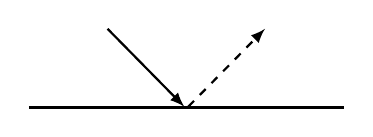
\begin{tikzpicture}
                  \draw[thick] (-2,0) -- (2,0);
                  \draw[thick, -latex] (-1,1) -- (-0.025,0.01);
                  \draw[thick, -latex, dashed] (0.025,0.01) -- (1,1);
              \end{tikzpicture}
          \end{center}





    \item \textbf{Diffrazione}: quando il segnale è ostruito da oggetti con superfici taglienti e irregolari, parte del segnale può modificare l'angolo con cui si propaga. Questo fenomeno permette in certe condizioni di ricevere un segnale anche in assenza di una linea di vista a causa di un oggetto che crea una zona d'ombra, ovviamente l'energia ricevuta sarà minore rispetto a quella originaria del segnale.
          \begin{center}
              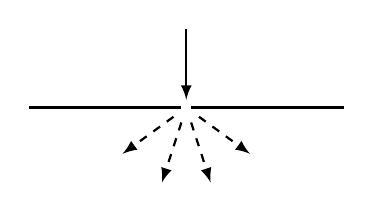
\begin{tikzpicture}
                  \draw[thick] (-2,0) -- (-0.0625,0);
                  \draw[thick] (0.0625,0) -- (2,0);
                  \draw[thick, -latex] (0,1) -- (0,0.1);

                  \draw[thick, -latex, dashed] (-0.1618033988749895, -0.1175570504584946) -- (-0.8090169943749476, -0.587785252292473);
                  \draw[thick, -latex, dashed] (-0.061803398874989514, -0.1902113032590307) -- (-0.30901699437494756, -0.9510565162951535);
                  \draw[thick, -latex, dashed] (0.061803398874989444, -0.19021130325903074) -- (0.30901699437494723, -0.9510565162951536);
                  \draw[thick, -latex, dashed] (0.16180339887498946, -0.11755705045849467) -- (0.8090169943749473, -0.5877852522924734);
              \end{tikzpicture}
          \end{center}



    \item \textbf{Scattering}: il segnale impatta con oggetti di piccola dimensione rispetto alla lunghezza d'onda si ha una propagazione in più direzioni del segnale, a differenza della diffrazione dove c'è più o meno una direzione comune dove il segnale va.
          \begin{center}
              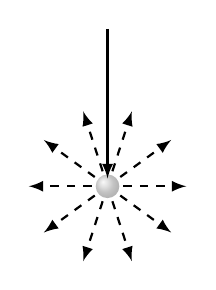
\begin{tikzpicture}
                  \shade[ball color=black!40, opacity=0.4] (0,0) circle (0.15cm);
                  \draw[thick, -latex] (0,2) -- (0,0.1);
                  \draw[thick, -latex, dashed] (0.16180339887498948, 0.11755705045849463) -- (0.8090169943749475, 0.5877852522924731);
                  \draw[thick, -latex, dashed] (0.06180339887498949, 0.1902113032590307) -- (0.30901699437494745, 0.9510565162951535);
                  \draw[thick, -latex, dashed] (-0.061803398874989465, 0.19021130325903074) -- (-0.30901699437494734, 0.9510565162951536);
                  \draw[thick, -latex, dashed] (-0.16180339887498946, 0.11755705045849466) -- (-0.8090169943749473, 0.5877852522924732);
                  \draw[thick, -latex, dashed] (-0.2, 2.4492935982947065e-17) -- (-1.0, 1.2246467991473532e-16);
                  \draw[thick, -latex, dashed] (-0.1618033988749895, -0.1175570504584946) -- (-0.8090169943749476, -0.587785252292473);
                  \draw[thick, -latex, dashed] (-0.061803398874989514, -0.1902113032590307) -- (-0.30901699437494756, -0.9510565162951535);
                  \draw[thick, -latex, dashed] (0.061803398874989444, -0.19021130325903074) -- (0.30901699437494723, -0.9510565162951536);
                  \draw[thick, -latex, dashed] (0.16180339887498946, -0.11755705045849467) -- (0.8090169943749473, -0.5877852522924734);
                  \draw[thick, -latex, dashed] (0.2, -4.898587196589413e-17) -- (1.0, -2.4492935982947064e-16);
              \end{tikzpicture}
          \end{center}






    \item \textbf{Assorbimento e rifrazione}: si tratta di fenomeni meno importanti, ma che comunque possono modificare la propagazione del segnale.
\end{itemize}

Gli effetti generati da questi fenomeni possono essere riassunti in due diversi tipi di attenuazione del segnale:
\begin{itemize}
    \item \textbf{Small-scale fading}: modella fluttuazioni rapide della potenza del segnale su lunghezze paragonabili a quella dell'onda.
    \item \textbf{Large-scale fading}: modella la variazione della potenza del segnale su lunghe distanze. Contribuisce al valore medio della potenza del segnale per una distanza di circa 1 m, e quindi verrà considerata come costante per distanze di circa 1 m.
\end{itemize}


\begin{center}
    \begin{forest}
        for tree={
        rectangle,
        draw,
        minimum size=1.75em,
        align=center,
        font=\scriptsize,
        s sep=1.5cm,
        l sep=1cm,
        edge={draw, semithick}
        }
        [Fading Types
            [Large Scale Fading
                    [Path Loss]
                    [Shadowing]
            ]
            [Small Scale Fading
                    [Multipath\\ delay spread
                            [Flat Fading]
                            [Frequency\\ Selective\\ Fading]
                    ]
                    [Doppler\\ spread
                            [Fast\\ Fading]
                            [Slow\\ Fading]
                    ]
            ]
        ]
    \end{forest}
\end{center}

\subsection*{Large-scale fading}
Il LSF modella la variazione della potenza del segnale in base alla distanza fra trasmettitore e ricevitore, tipicamente variando per distanze nell'ordine del metro. Gli effetti sono modellati attraverso la combinazione di \textbf{path loss} e \textbf{shadowing}:

\paragraph*{Path Loss}
Il path loss è un valore deterministico che modella la media dell'attenuazione della potenza ricevuta, rappresenta un'approssimazione delle equazioni di Maxwell.
È la grandezza che maggiormente dipende dalla distanza tra trasmettitore e ricevitore nel fading.
\begin{equation}
    P_{RX} \approx P_{TX} \cdot \Gamma(f_0, d_0) \cdot \left( \frac{d_0}{d} \right)^n \quad \text{for } d > d_0
\end{equation}
dove \( \Gamma(f_0, d_0) \approx \left( \frac{\lambda_0}{4 \pi d_0} \right)^2 \) rappresenta il termine di campo vicino, \( P_{TX} \) è la potenza trasmessa, \( d_0 \) è la distanza di riferimento e \( n \) è l'esponente del path loss. Quest'ultimo dipende dall'ambiente in cui ci si trova, ad esempio in un ambiente urbano il valore di \( n \) varia tra 2.7 e 3.5.
\begin{table}[h!]
    \centering
    \begin{tabular}{|>{\raggedright}p{4cm}|>{\centering\arraybackslash}p{2cm}|}
        \hline
        \textbf{Environment}             & \textbf{Path Loss Exponent, \( n \)} \\
        \hline
        Free space                       & 2                                    \\
        \hline
        Urban area cellular radio        & 2.7 -- 3.5                           \\
        \hline
        Urban area cellular (obstructed) & 3 -- 5                               \\
        \hline
        In-building line-of-sight        & 1.6 -- 1.8                           \\
        \hline
        Obstructed in-building           & 4 -- 6                               \\
        \hline
        Obstructed in-factories          & 2 -- 3                               \\
        \hline
    \end{tabular}
    \caption{Esponenti del path loss per vari ambienti}
\end{table}

Se abbiamo un'antenna, possiamo assumere che esista un'area di raggio $d_0$ centrata nell'antenna, che non è ostruita, mentre $d$ rappresenta la distanza tra l'area di raggio $d_0$ e il ricevitore, lungo cui ci invece sono ostacoli. In questa area si calcola l'attenuazione utilizzando la regola come se si fosse nello spazio vuoto.
Il valore di \( d_0 \) è scelto in modo da poter misurare o stimare con precisione il path loss in condizioni controllate, in modo da poter avere un punto di riferimento da cui calcolare le perdite aggiuntive a distanze maggiori.
In reti cellulari che coprono aree estese si utilizza una distanza di riferimento di 1 km, mentre in reti progettate per aree più piccole e densamente popolate si utilizzano distanze di riferimento di 100 metri o anche 1 metro.

\begin{center}
    \resizebox{0.5\textwidth}{!}{
        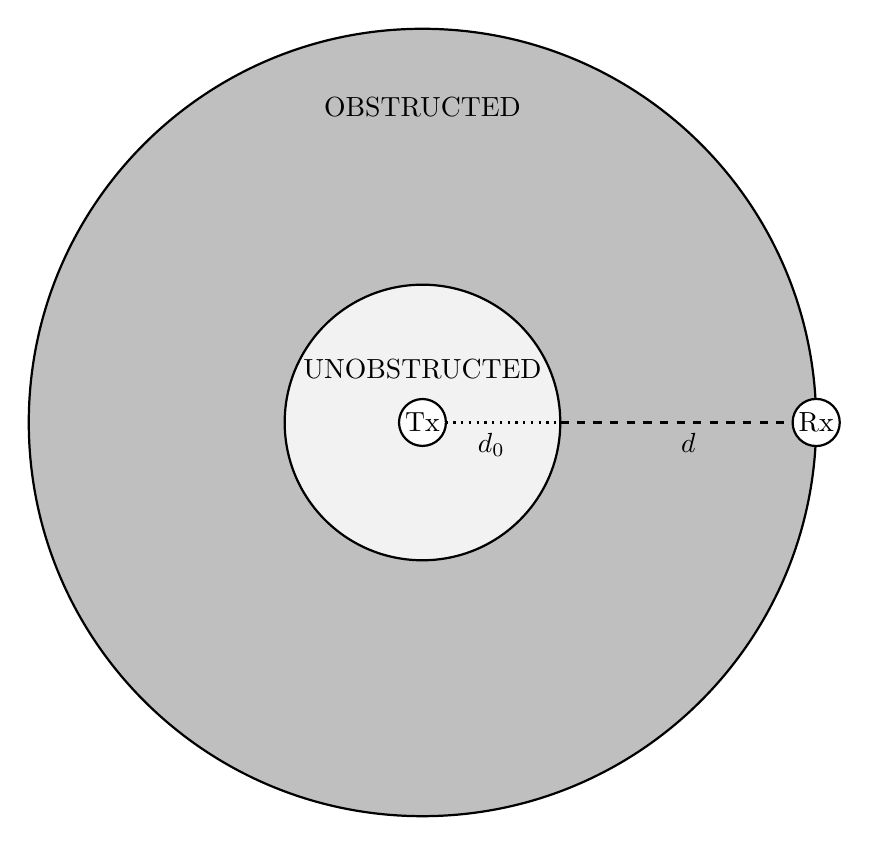
\begin{tikzpicture}[
                thick,
                txt/.style={circle, inner sep=1pt, fill=white, draw=black},  % Reduced text size for Tx and Rx
                line/.style={thick, dashed, gray},
                dotted2/.style={thick, dotted, gray},  % New style for dotted lines
                label distance=3pt
            ]
            % Define central point
            \coordinate (O) at (0,0);

            % Drawing the outer "obstructed" area with light gray fill and horizontal lines
            \draw[fill=gray!50] (O) circle[radius=5cm];
            % Labeling the outer circle
            \node at (0,4) {OBSTRUCTED};  % Reduced text size and positioned within the circle

            % Drawing the inner "unobstructed" area with darker gray fill
            \draw[fill=gray!10] (O) circle[radius=1.75cm];
            % Labeling the inner circle
            \node at (0,0.675) {UNOBSTRUCTED};  % Reduced text size and positioned within the circle

            % Central transmitter node

            % Dashed line indicating radius
            \draw[dotted] (O) -- (1.75,0) node[midway, below] {$d_0$};

            % Dotted line replacing the second dashed line
            \draw[dashed] (1.75,0) -- (5,0) node[midway, below] {$d$};

            \node[txt] at (O) {Tx}; % Shifted below the center
            % Arrow indicating receiver
            \node[txt] at (5,0) {Rx}; % Shifted below the line end

        \end{tikzpicture}
    }
\end{center}

La formula, deterministica, che fornisce il valore di attenuazione data dal path loss è:
\[
    A_{PL} = \frac{P_{RX}}{P_{TX}} = \Gamma(f_0, d_0) \cdot \left( \frac{d_0}{d} \right)^n
\]
\[
    A_{PL}^{dB} = P_{RX}^{dB} - P_{TX}^{dB}
\]
\[
    A_{PL}^{dB} = 10 \cdot \log_{10}(A_{PL}) = \Gamma(f_0, d_0)_{dB} + n \cdot 10 \cdot \log_{10}(d_0) - n \cdot 10 \cdot \log_{10}(d)
\]


Nel vuoto l'attenuazione del segnale in base alla distanza è data dalla relazione
\[
    P_{RX} = P_{TX} \cdot \frac{A}{4\pi d^2}
\]
dove \( A \) è l'area dell'antenna in ricezione, che tipicamente è \( A = \lambda^2 \) dove \( \lambda \) è la lunghezza d'onda del segnale.


Per frequenze inferiori a 6 GHz l'attenuazione dipende dalle frequenze con una relazione quadratica, tuttavia oltre tale soglia la lunghezza d'onda è sufficientemente piccola per interagire con molecole presenti nell'aria, in particolare ossigeno e vapore acqueo, incrementando ulteriormente l'attenuazione.

Nella progettazione di sistemi di comunicazione wireless è essenziale tenere in considerazione il rapporto tra frequenza utilizzata e distanza copribile da una singola antenna.
Il path loss è causato anche dalle frequenze più elevate: una frequenza alta significa una lunghezza d'onda piccola, quindi alcuni materiali possono risultare opachi ai campi elettromagnetici, diventando praticamente degli ostacoli.
Questo implica che più alta è la frequenza utilizzata, più celle sono necessarie per coprire una determinata area, perché l'area in cui l'attenuazione è accettabile si riduce.
Per avere una copertura maggiore è meglio utilizzare frequenze portanti minori (si avranno celle grandi), ma per avere capacità maggiori si usano frequenze più alte perché lo spettro disponibile è maggiore (si avranno celle piccole).

\paragraph*{Shadowing}

Dati due punti alla stessa distanza dal trasmettitore, se si considerasse unicamente il path loss, si avrebbe la stessa attenuazione,
tuttavia nella realtà vi è una componente aleatoria da dover considerare, modellabile tramite shadowing.
La componente aleatoria è dovuta alla presenza di ostacoli differenti che coprono parzialmente il segnale ricevuto ed è caratterizzata da una distribuzione log-normale con parametri $\mu = 0$ e $\sigma_S$, espressi in dB, quindi una distribuzione normale con parametri ($A_S$ e $\sigma_S$) espressi in dB,
ovvero la PDF è:
\[
    f_{A_s^{dB}}(a_S) = \frac{1}{\sqrt{2\pi \sigma_S^2}} e^{-\frac{a_S^2}{2\sigma_S^2}}
\]
Tipicamente $\sigma_S$ varia tra 0 e 9 dB.
Gli effetti del path loss e dello shadowing sono sommati per ottenere le variazioni dovute al large scale fading.
\[
    A_{LS} = A_{PL} \cdot A_S \quad \text{scala lineare}
\]

\[
    A_{LS}^{dB} = A_{PL}^{dB} + A_S^{dB} \quad \text{scala logaritmica}
\]
Entrambi contribuisoono a variazioni nella potenza media ricevuta, le cui fluttuazioni sono significative solo per grandi distanze, considerando la lunghezza d'onda.

\begin{center}
    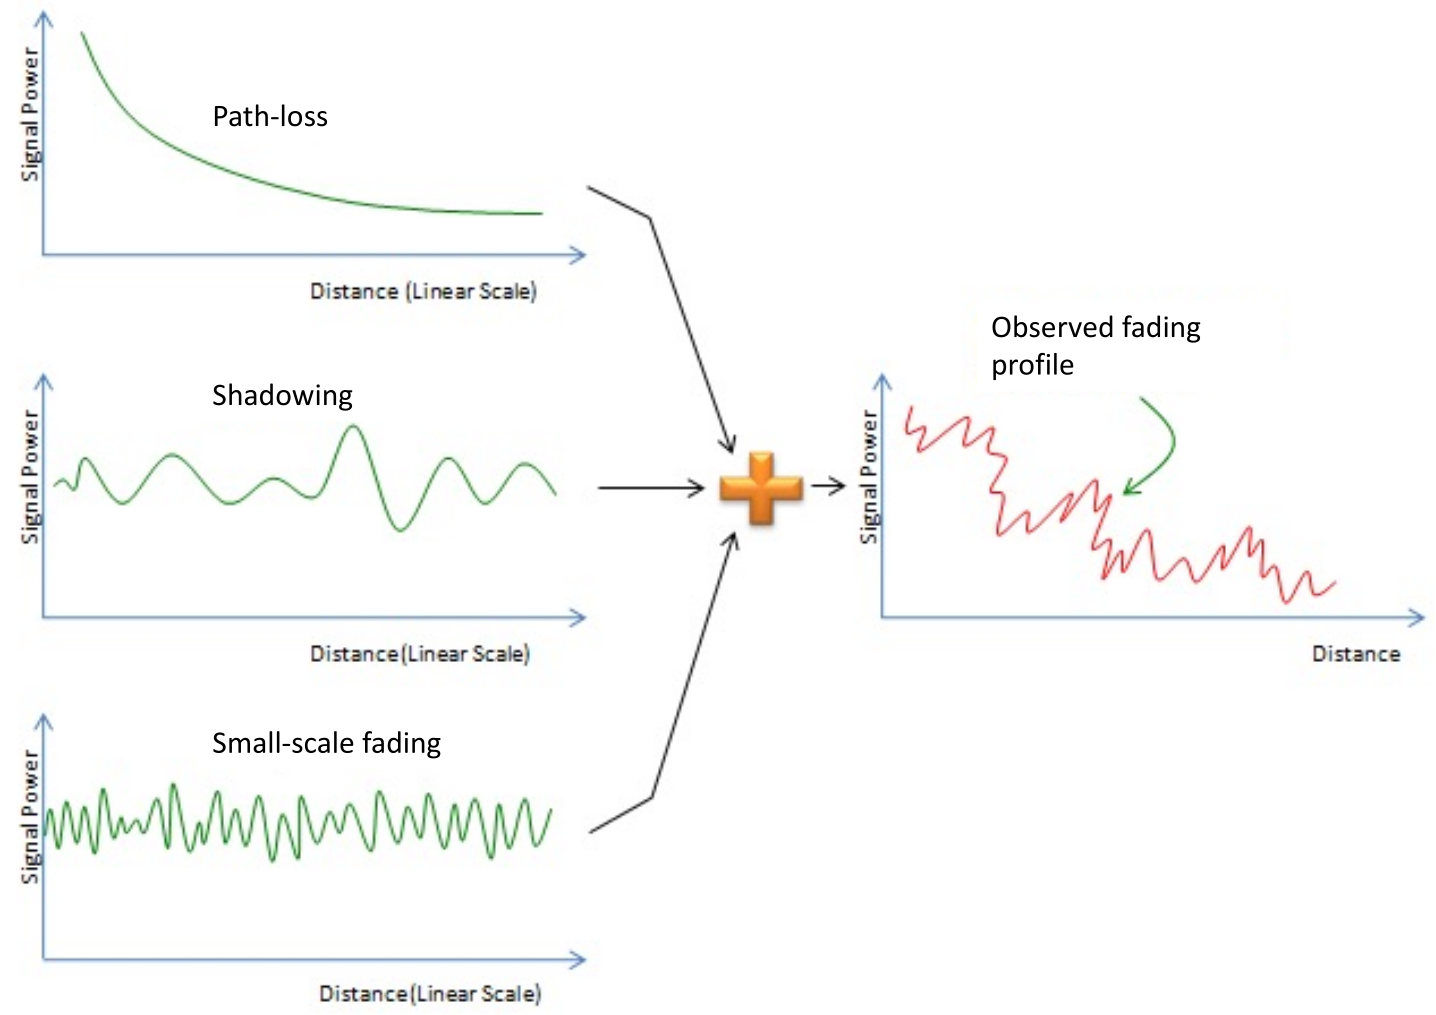
\includegraphics[width=0.675\textwidth]{imgs/fading_sum.jpg}
\end{center}
\section*{Small scale fading}

Lo small scale fading modella le variazioni aleatorie della potenza istantanea su distanze nell'ordine della lunghezza d'onda, dovute ai vari fenomeni di propagazione delle onde che determinano la ricezione di repliche del segnale, ognuno con un certo ritardo, fase ed attenuazione.
Il canale di tramissione è modellato come un filtro LTI, la cui risposta impulsiva dipende dagli effetti SSF:

\[
    h(t) = A_{LS} \sum_{\ell=0}^{N_c-1} \alpha_{\ell} e^{j\phi_{\ell}} \delta(t - \tau_{\ell})
\]

Dove \( A_{LS} \) è l'attenuazione dovuta al large scale fading (quindi path loss e shadowing), \( \alpha_{\ell} \) e \( \phi_{\ell} \) sono rispettivamente ampiezza e fase del segnale \(\ell\)-esimo, e \( \tau_{\ell} \) è il ritardo temporale.
% TODO: questa frase sotto non è chiara
% TODO: c'è una relazione tra %phi_l e tau_l? 
La diversa fase è dovuta al fatto che il segnale è modulato con la frequenza della portante, quindi se c'è una piccola differenza di tempo nell'arrivo, ci sarà anche una diversa rotazione dovuta alla frequenza della portante.
La risposta impulsiva del canale è la somma delle risposte impulsiva di ogni singolo percorso.

Per quanto riguarda i parametri delle varie repliche:
\begin{itemize}
    \item \textbf{Attenuazioni} ($\alpha_\ell$): sono modellate come variabili aleatorie, tipicamente con distribuzione di Rayleigh, derivante dal fatto che le componenti in fase e quadratura hanno una distribuzione normale.
          \[
              \alpha e^{j\phi_i} = x_i + j y_i \quad \text{con } x_i, y_i \sim \mathcal{N}(0, \sigma^2)
          \]
          % TODO: il primo passaggio sotto non torna
          \[
              \alpha = \|\alpha e^{j\phi_i}\| = \sqrt{x_i^2 + y_i^2} \sim \text{Rayleigh}(\sigma)
          \]

          \begin{itemize}
              \item La distribuzione per l'ampiezza del canale \(\alpha\) è \textit{Rayleigh}\footnote{
                        Siano \(X\) e \(Y\) variabili casuali normali indipendenti con media 0 e varianza \(\sigma^2\). La pdf congiunta di \(X\) e \(Y\) è data da:
                        \[
                            f_{X,Y}(x,y) = \frac{1}{2\pi\sigma^2} \exp\left(-\frac{x^2 + y^2}{2\sigma^2}\right).
                        \]
                        Per cui la CDF della variabile aleatoria \( R = \sqrt{X^2 + Y^2}\) è data da:
                        \[
                            F_R(r) = \int_{x^2 + y^2 < r^2} \frac{1}{2 \pi \sigma^2} e^{-\frac{x^2 + y^2}{2\sigma^2}} \, dx \, dy
                        \] 
                        


                        Passando alle coordinate polari, lo Jacobiano della trasformazione dalle coordinate cartesiane \((x, y)\) alle coordinate polari \((\rho, \theta)\) è \(\rho\), cioè:
                        \[
                            dx \, dy = \rho \, d\rho \, d\theta.
                        \]
                        La CDF diventa quindi:
                        \[
                            F_R(r) = \int_{\rho < r, 0 \leq \theta \leq 2\pi} \frac{1}{2 \pi \sigma^2} e^{-\frac{\rho^2}{2\sigma^2}} \rho \, d\rho \, d\theta = \int_{0}^{2\pi} d\theta \int_{0}^{r} \frac{\rho}{2\pi \sigma^2} e^{-\frac{\rho^2}{2\sigma^2}}\, d\rho = \int_{-\infty}^{r} \frac{\rho}{\sigma^2} e^{-\frac{\rho^2}{2\sigma^2}} \text{u}(\rho)\, d\rho
                        \] 
                        Ovvero:
                        \[
                            f_R(r) = \frac{r}{\sigma^2} e^{-\frac{r^2}{2\sigma^2}} \text{u}(r)
                        \]
                    }
                    \[
                        f_{\alpha}(x) = \frac{x}{\sigma^2} e^{-\frac{x^2}{2\sigma^2}} \text{u}(x)
                    \]

              \item La distribuzione per la potenza del canale \(s = \alpha^2\) è \textit{esponenziale}\footnote{Sapendo che la PDF di $\alpha$ è $f_{\alpha}(x) = \frac{x}{\sigma^2} e^{-\frac{x^2}{2\sigma^2}} \text{u}(x)$, possiamo calcolare la PDF di $s = \alpha^2$:
                \[
                    F_{\alpha}(x) = \mathbb{P}\left\{ \alpha \leq x \right\} = \int_{0}^{x} \frac{t}{\sigma^2} e^{-\frac{t^2}{2\sigma^2}} \, dt
                \]
                Ovvero:
                \[
                    \mathbb{P}\left\{ s \leq x^2 \right\} = \mathbb{P}\left\{ \alpha^2 \leq x^2 \right\} = \int_{0}^{x^2} \frac{t}{\sigma^2} e^{-\frac{t}{2\sigma^2}} \, dt
                \]
                Applicando il cambio di variabile $t^2 = u$:
                \[
                     \mathbb{P}\left\{ s \leq x^2 \right\} = \int_{0}^{x} \frac{1}{2\sigma^2} e^{-\frac{u}{2\sigma^2}} \, du 
                \]
                Ovvero, per il primo teorema fondamentale del calcolo integrale, la derivata della CDF di $s$ è:
                \[
                    f_s(x) = \frac{1}{2\sigma^2} e^{-\frac{x}{2\sigma^2}} \text{u}(x)
                \]
                
                

            }

                    \[
                        %f_s(s) =
                       % \begin{cases}
                       %     \frac{1}{2\sigma^2} e^{-\frac{s}{2\sigma^2}} & s \geq 0 \\
                      %      0                                            & s < 0
                       % \end{cases}
                        f_s(s) = \frac{1}{2\sigma^2} e^{-\frac{s}{2\sigma^2}} \text{u}(s)
                    \]
          \end{itemize}

    \item \textbf{Fasi} ($\phi_\ell$): sono modellate come variabili distribuite uniformemente nell'intervallo $[0, 2\pi]$.
\end{itemize}

La ricezione di più repliche, soprattutto se notevolmente distanziate tra loro, genera ISI.
\[
    x(t) = \sum_{i} c_i g(t - iT) \quad \text{uscita filtro in ricezione (senza rumore)}
\]
\[
    g(t) = g_T(t) \ast h(t) \ast g_R(t) = g_N(t) \ast h(t) = \sum_{\ell=0}^{N_c-1} \alpha_{\ell} e^{j\phi_{\ell}} g_N(t - \tau_{\ell})
\]
\[
    g\left[k\right] = \sum_{\ell=0}^{N_c-1} \alpha_{\ell} e^{j\phi_{\ell}} g_N\left(kT - \tau_{\ell}\right)
\]

\[
    x\left[m\right] = \sum_{k=-\infty}^{+\infty} c_k g\left[m - k \right] = c_m g(0) + \sum_{\substack{k \neq m,\\ k=-\infty}}^{+\infty} c_{k} g\left[m-k\right]
\]


Sebbene quindi si scelga un filtro che rispetti la condizione di Nyquist, gli effetti del canale non permettono di rimuovere completamente l'ISI, generata dal fatto che $g\left[m-k\right]$ non si annulla.


Definiamo dei parametri che ci permettano di capire la gravità dell'ISI.
Il delay spread, che può essere interpretato come la differenza di tempo tra l'istante d'arrivo della prima componente del multipath e l'istante d'arrivo dell'ultima, permette di misurare la dispersione temporale introdotta dal canale:
\begin{itemize}
    \item $\sigma_\tau \ll T$: delay spread inferiore al symbol time, il canale è detto \textbf{flat fading}  e l'effetto dell'ISI è trascurabile in quanto le varie repliche ricevute fanno tutte riferimento allo stesso simbolo.
    \item $\sigma_\tau > T$: delay spread maggiore del symbol time, il canale è detto \textbf{frequency selective} e l'effetto dell'ISI non è più trascurabile in quanto le varie repliche, appartenti a simboli differenti, interferiscono tra loro.
\end{itemize}

\begin{center}
    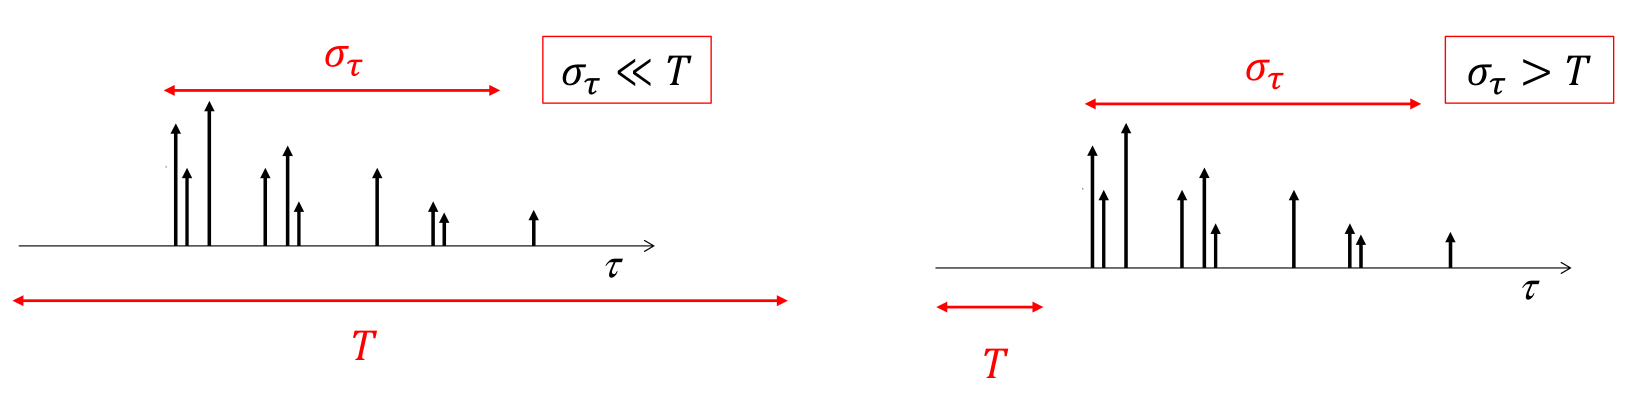
\includegraphics[width=0.75\textwidth]{imgs/delay_spread.png}
\end{center}


\noindent
\begin{minipage}{.5\textwidth}
    \centering
    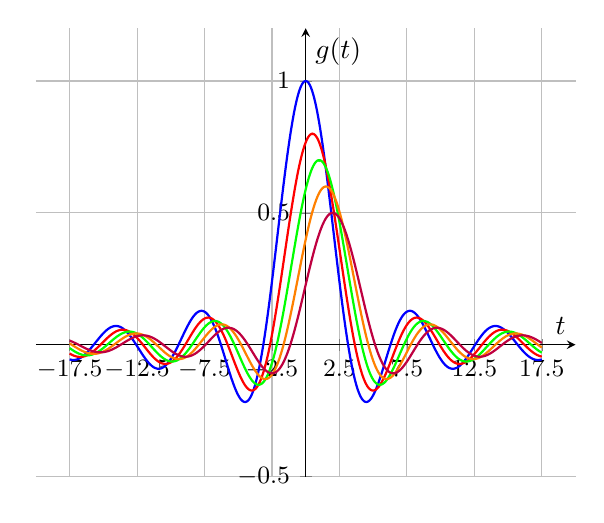
\begin{tikzpicture}
        \begin{axis}[
                axis lines = middle,
                xlabel = \(t\),
                ylabel = {\(g(t)\)},
                grid=major,
                domain=-17.5:17.5,  % updated domain
                samples=1000,
                ymin=-0.5, ymax=1.2,
                xmin=-20, xmax=20,  % adjusted for better visibility
                xtick={-17.5, -12.5, ..., 17.5},  % updated ticks
                ytick={-0.5, 0, ..., 1},
                ticklabel style={font=\small},
                legend pos=north east,
                legend style={nodes={scale=0.8, transform shape}}
            ]
            \addplot[blue, thick] {sin(deg(x))/x};
            \addplot[red, thick] {0.8*sin(deg(x - 0.5))/(x - 0.5)};
            \addplot[green, thick] {0.7*sin(deg(x - 1))/(x - 1)};
            \addplot[orange, thick] {0.6*sin(deg(x - 1.5))/(x - 1.5)};
            \addplot[purple, thick] {0.5*sin(deg(x - 2))/(x - 2)};

        \end{axis}
    \end{tikzpicture}
\end{minipage}
\begin{minipage}{.5\textwidth}
    \centering
    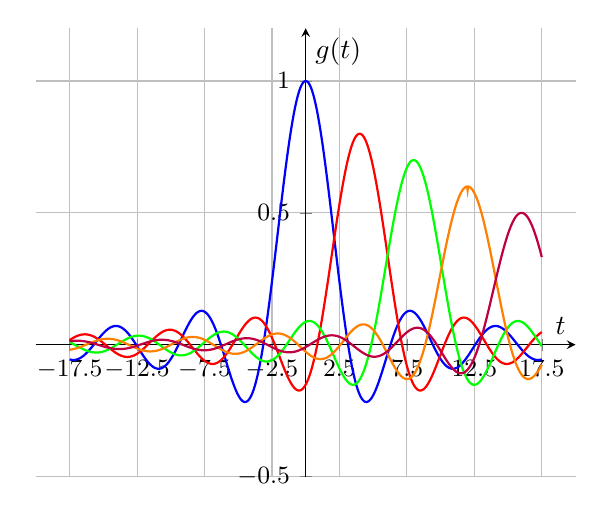
\begin{tikzpicture}
        \begin{axis}[
                axis lines = middle,
                xlabel = \(t\),
                ylabel = {\(g(t)\)},
                grid=major,
                domain=-17.5:17.5,  % updated domain
                samples=1000,
                ymin=-0.5, ymax=1.2,
                xmin=-20, xmax=20,  % adjusted for better visibility
                xtick={-17.5, -12.5, ..., 17.5},  % updated ticks
                ytick={-0.5, 0, ..., 1},
                ticklabel style={font=\small},
                legend pos=north east,
                legend style={nodes={scale=0.8, transform shape}}
            ]
            \addplot[blue, thick] {sin(deg(x))/x};
            \addplot[red, thick] {0.8*sin(deg(x - 4))/(x - 4)};
            \addplot[green, thick] {0.7*sin(deg(x - 8))/(x - 8)};
            \addplot[orange, thick] {0.6*sin(deg(x - 12))/(x - 12)};
            \addplot[purple, thick] {0.5*sin(deg(x - 16))/(x - 16)};

        \end{axis}
    \end{tikzpicture}
\end{minipage}


In entrambi i casi il canale è detto \textbf{multipath} in quanto la ricezione del segnale avviene attraverso più repliche, a cui poi si aggiunge una classificazione ulteriore dovuta al delay spread.
Nel caso flat fading essendo le repliche molto vicine è ragionevole l'approssimazione a una sola replica e quindi siamo in una situazione con una piccola ISI, nel caso invece multipath questa assunzione non vale e l'ISI è grande.
Invece che utilizzare il delay spread si può utilizzare, in frequenza, la \textbf{coherence bandwidth}, definita come l'intervallo di frequenze per cui la risposta in frequenza del canale è circa costante:
\[
    B_c \approx \frac{1}{5\sigma_\tau}
\]
Se $B_c > B_S \approx \frac{1}{T}$, ovvero la banda del segnale trasmesso, non si avrà alcune distorsione, il canale risulta \textbf{flat fading}. In caso contrario, se $B_c < B_S$ il canale è detto \textbf{frequency selective}.
\begin{center}
    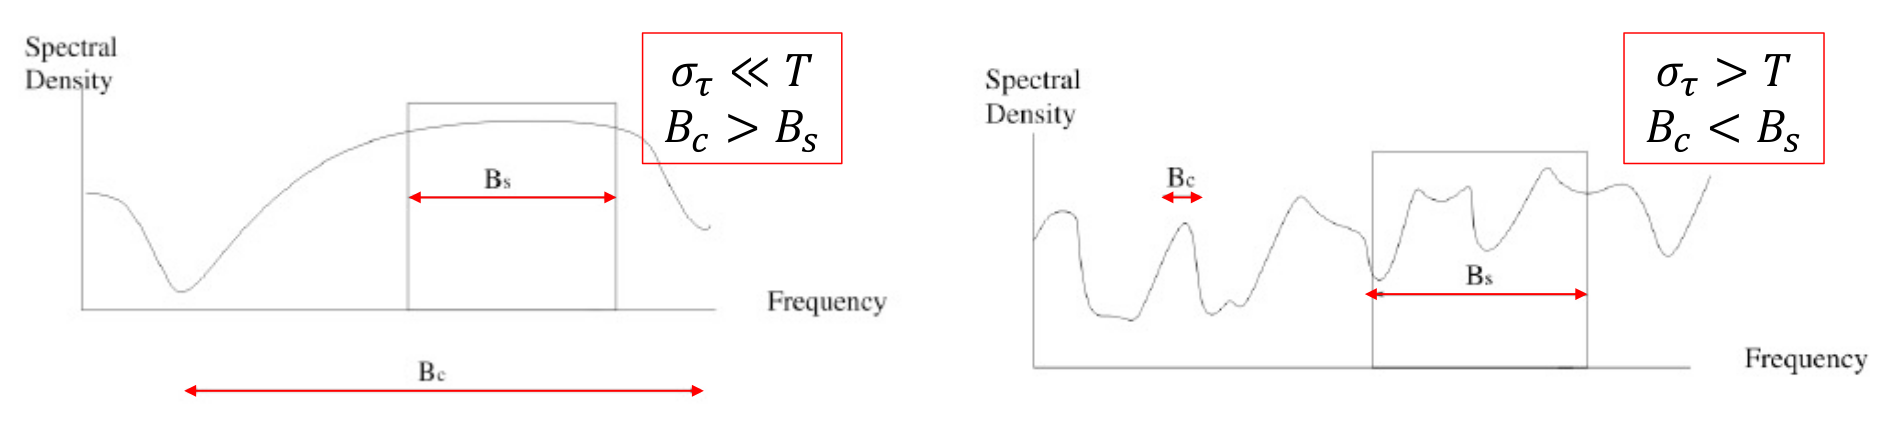
\includegraphics[width=0.875\textwidth]{imgs/coherence_bandwidth.png}
\end{center}
La coherence bandwidth può essere determinata considerando la densità spettrale di potenza.
%TODO questa parte non è chiara.
Quando $\sigma_{\tau} < T$ vale $B_c > B_s$ e il canale è flat fading, altrimenti se $\sigma_{\tau} > T$ vale $B_c < B_s$ e il canale è frequency selective.
I delay sono modellabili come variabili aleatorie $\tau$, perché per ottenere proprietà statistiche si possono applicare le operazioni standard per il calcolo del valore medio e della varianza, tuttavia ciò risulta particolarmente complesso e serve dunque approssimare.


\[
    \overline{\tau} = \mathbb{E} \left[\tau\right] = \int_{-\infty}^{+\infty} \tau f_{\tau}(\tau) d\tau \approx \sum_{\ell=0}^{N_c-1} \frac{\alpha_{\ell}^2}{\sum_{m=0}^{N_c-1} \alpha_{m}^2} \tau_{\ell}
\]

Per quanto riguarda la varianza:
\[
    \sigma_\tau^2 = \mathbb{E}\left[({\tau - \overline{\tau}})^2\right] \approx \overline{\tau^2} - \overline{\tau}^2, \quad \overline{\tau^2} = \mathbb{E} \left[\tau^2\right] = \int_{-\infty}^{+\infty} \tau^2 f_{\tau}(\tau) d\tau \approx \sum_{\ell=0}^{N_c-1} \frac{\alpha_{\ell}^2}{\sum_{m=0}^{N_c-1} \alpha_{m}^2} \tau_{\ell}^2
\]

Per modellare gli effetti di small scale fading si utilizza il parametro $\sigma_\tau$, ovvero il delay spread che dipende dall'ambiente in cui avviene la trasmissione. Il modello ottenuto risulta piuttosto semplice da utilizzare e scegliendo accuratamente i parametri può essere utilizzato per modellare diversi scenari di trasmissione. L'accuratezza ottenuta non è sempre fedele al caso reale, ma nella maggior parte dei casi non è richiesto, considerando anche che il canale è soggetto a cambiamenti repentini.

Il BER a parità di rumore dipende fortemente dalla distorsione introdotta nel canale:
\begin{itemize}
    \item \textbf{No fading}: aumentando il rapporto segnale/rumore (SNR) è possibile ridurre drasticamente il BER con una potenza di trasmissione contenuta.
    \item \textbf{Flat fading}: aumentando il rapporto segnale/rumore (SNR) è ancora possibile ridurre il BER, ma sarà necessaria una potenza di trasmissione maggiore.
    \item \textbf{Frequency selective}: il BER non è riducibile oltre una certa soglia nonostante l'incremento del SNR, principalemente a causa delle interferenze generate dall'ISI.
\end{itemize}

Per quanto riguarda le variabili decisionali:
\[
    x\left[m\right] = c_m + n\left[m\right] \quad \text{no fading} \quad P_e = Q(\sqrt{\text{SNR}})
\]

\[
    x\left[m\right] = \alpha \cdot c_m + n\left[m\right] \quad \text{flat fading} \quad P_e = \frac{1}{\text{SNR}}
\]

\[
    x\left[m\right] = c_m g(0) + \sum_{\substack{k \neq m,\\ k=-\infty}}^{+\infty} c_{k} g\left[m-k\right] + n\left[m\right] \quad \text{frequency selective}
\]

Nell'ultimo caso, inizialmente è il rumore a dominare, quindi incrementando la potenza di trasmissione si ottengono miglioramenti nel BER, tuttavia così facendo si incrementa anche l'energia dei simboli finendo in una zona in cui è l'ISI a dominare.
La tendenza delle nuove generazioni radio è quella di incrementare il symbol-time. Questo comporta il rischio di ottenere con più facilità canali frequency selective anche in ambienti non particolarmente ostili. Per questo le classiche modulazioni PAM o QAM non risultano adatte in certi contesti, ma si fa uso di nuove tipologie di modulazioni multi-carrier come OFDM.


Le misurazioni del canale dipendono dalla frequenza del segnale e dall'ambiente in cui avviene la trasmissione.
%Typical values of delay spread are:
Valori tipici di delay spread sono:

\begin{itemize}
    \item $0.2 \, \si{\mu s}$ (area rurale),
    \item $0.5 \, \si{\mu s}$ (area suburbana),
    \item $3-8 \, \si{\mu s}$ (area urbana),
    \item $<2 \, \si{\mu s}$ (microcella urbana),
    \item $50-300 \, \si{ns}$ (picocella indoor).
\end{itemize}

\begin{center}
    \begin{tabular}{|c|c|c|}
        \hline
        \textbf{Ambiente} & \textbf{RMS Delay Spread ($\sigma_\tau$)}       & \textbf{Note}      \\
        \hline
        Urbano            & $1300 \, \si{ns} \, (3500 \, \si{ns} \text{ max})$  & NYC                \\
        LTE ETU           & Fino a $5 \, \si{\mu s}$                             & Caso tipico medio  \\
        Suburbano         & $1960-2110 \, \si{ns}$                        & Caso estremo medio \\
        Indoor            & $10-50 \, \si{ns}$                            & Edificio d'uffici  \\
        Indoor            & $70-94 \, \si{ns} \, (1470 \, \si{ns} \text{ max})$ & Edificio d'uffici  \\
        \hline
    \end{tabular}
\end{center}


Per esempio, in un'area urbana con delay spread $\sigma_\tau = 4 \mu s$, avremo una coherence bandwidth di $B_c \approx \frac{1}{5 \sigma_\tau} = \frac{1}{20 \mu s} = 50 \text{kHz}$.

\section*{Time varying channel}
Se il ricevitore di un segnale è in movimento il modello di canale risulta più complesso, in quanto è necessario aggiungere una dipendenza dal tempo ai guadagni e alle fasi alle varie repliche.
Intuitivamente tali dipendenze dipendono dal fatto che gli effetti di small scale fading variano drasticamente anche per distanze paragonabili alla lunghezza d'onda, le quali possono essere nell'ordine del centimetro.
Tipicamente il canale è descritto come sistema LTI in modo da poter sfruttare la sua risposta impulsiva, ma nel caso di ricevitore mobile vi è una dipendenza dal tempo.
Tuttavia nella maggior parte dei casi pratici l'assunzione LTI risulta valida.

% TODO: inserire considerazione sulla BER
% TODO: %\delta(t - \tau) o \delta(\tau - \tau_l
\[
    h(t) = A_{LS} \sum_{\ell=0}^{N_c-1} \alpha_{\ell}(t) e^{j\phi_{\ell}(t)} \delta(t - \tau_{\ell})
\]
% TODO: mediato?
Dove abbiamo aggiunto la dipendenza dal tempo alle ampiezze e alle fasi delle repliche. Dato che il large scale fading è mediato su una distanza nell'ordine del metro, lo possiamo considerare costante (avendo un rate con cui varia molto più lento).
Anche per il ritardo non si aggiunge dipendenza dal tempo in quanto varia anch'esso molto più lentamente rispetto a guadagni e fasi, dato che le repliche viaggiano alla velocità della luce e quindi muoversi di pochi metri non ha un impatto significativo.


\subsection*{Effetto Doppler}
\begin{center}
    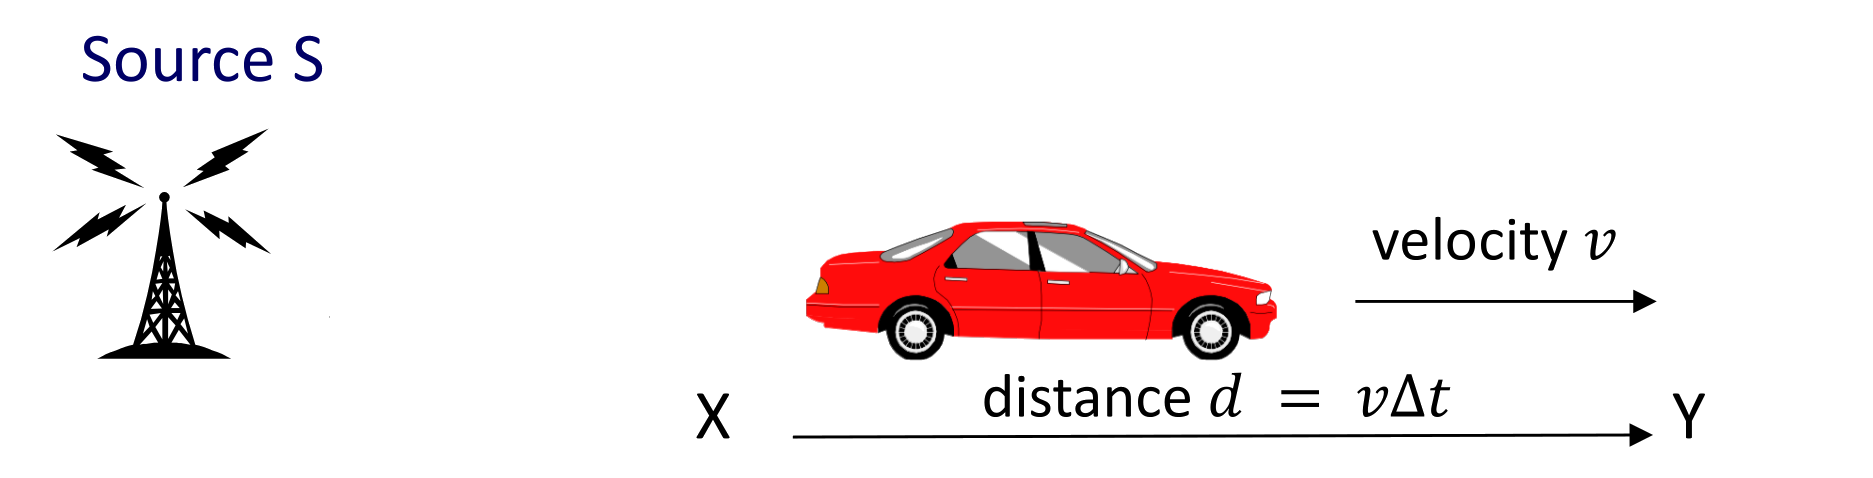
\includegraphics[width=0.75\textwidth]{imgs/doppler.png}
\end{center}

L'effetto Doppler, considerando una qualsiasi onda, è un fenomeno fisico che consiste nel cambiamento apparente della frequenza d'onda percepita da un osservatore raggiunto da un'onda emessa da una sorgente in movimento rispetto ad esso.
In particolare se la sorgente si avvicina la frequenza apparirà più elevata, mentre se si allontana sembrerà meno elevata, questo deriva dalla compressione (o allargamento) dei tempi in cui l'onda è ricevuta dall'osservatore.
Questo effetto ha delle implicazioni anche per quanto riguarda le onde radio utilizzate per le trasmissioni wireless, introducendo uno shift nelle frequenze del segnale ricevuto indicato come \textbf{Doppler shift} ($f_d$).
Lo shift può essere determinato considerando la velocità con cui si sta muovendo il ricevitore:
\[
    d = vt \quad \text{distanza tra $x$ e $y$}
\]

\[
    \Delta \tau = \frac{d}{c} = \frac{vt}{c} \quad \text{tempo impiegato dal segnale a percorrere $d$}
\]

\[
    y_x(t) = s(t) = \sin(2\pi f_c t) \quad \text{segnale ricevuto in $x$ al tempo $t$}
\]

\[
    y_y(t) = s(t-\Delta \tau) = \sin(2\pi f_c (t-\Delta \tau)) \quad \text{segnale ricevuto in $y$ al tempo $t$}
\]

\[
    = \sin\left(2\pi f_c \left(t - \frac{vt}{c}\right)\right) = \sin\left(2\pi \left(f_c - \frac{f_c v}{c}\right) t\right) = \sin\left(2\pi \left(f_c - f_d \right) t \right) \quad \boxed{f_d = -\frac{f_c v}{c}}
\]
Indicando con $f'$ la frequenza apparente percepita in $y$, ovvero $f_c - f_d$, vale la relazione:
\[
    f' = f_c - f_d = f_c \left(1 - \frac{v}{c}\right) = f_c \left( \frac{c - v}{c} \right)
\]
cioè un caso particolare della formula generale dell'effetto Doppler, ovvero
\[
    f' = f_c \left( \frac{c \pm v}{c \pm v_s} \right)
\]

dove:
\begin{itemize}
    \item $f$ è la frequenza trasmessa,
    \item $c$ è la velocità della luce,
    \item $v$ è la velocità del ricevitore rispetto al mezzo di propagazione,
    \item $v_s$ è la velocità della sorgente rispetto al mezzo di propagazione.
\end{itemize}


Il segno dipende dalla direzione del movimento, ovvero se la sorgente e l'osservatore si stanno avvicinando o allontanando.
Nell'esempio si assume che il ricevitore si stia allontanando dalla sorgente, quindi il segno è negativo, mentre il trasmettitore è fermo.
Il segnale ricevuto in $y$ risulta avere una frequenza inferiore a quello in $x$.
Il termine $f_d$ assume un valore significativo solo per $v$ o $f_c$ molto grandi, in quanto a denominatore si ha la velocità della luce.
In generale l'effetto introdotto non produce grandi errori, tuttavia nel caso di canale con introduzione di repliche si ha la ricezione di repliche con angoli differenti, generando un fenomeno più difficile da trattare e non deterministico, detto \textbf{Doppler spread}.
% TODO: theta è una variabile aleatoria?
Il Doppler shift di ciascuna replica dipende dall'angolo $\theta$, quindi $f_d = f_c \frac{v \cos(\theta)}{c}$.
Il segnale ricevuto invece viene descritto come un processo aleatorio a media nulla e se ne studia \textbf{autocorrelazione} e \textbf{densità spettrale di potenza}.
Esistono diversi modelli utilizzati per descrivere lo spreading in frequenza,
che si verifica quando le varie repliche del segnale vengono aggregate al ricevitore.

Tra questi modelli, il modello dello spettro Doppler di Jakes è particolarmente noto, il quale presuppone che le repliche del segnale arrivino in maniera uniformemente distribuita da ogni direzione, con ciascuna replica che apporta la stessa quantità di energia, cosicché nessuna direzione risulti favorita rispetto ad un'altra in termini di intensità del segnale ricevuto (\textit{scattering isotropico})
L'assunzione non è del tutto realistica, ma più che la forma dello spread è importante conoscere il fenomeno introdotto dal canale.

\begin{figure}[ht]
    \centering
    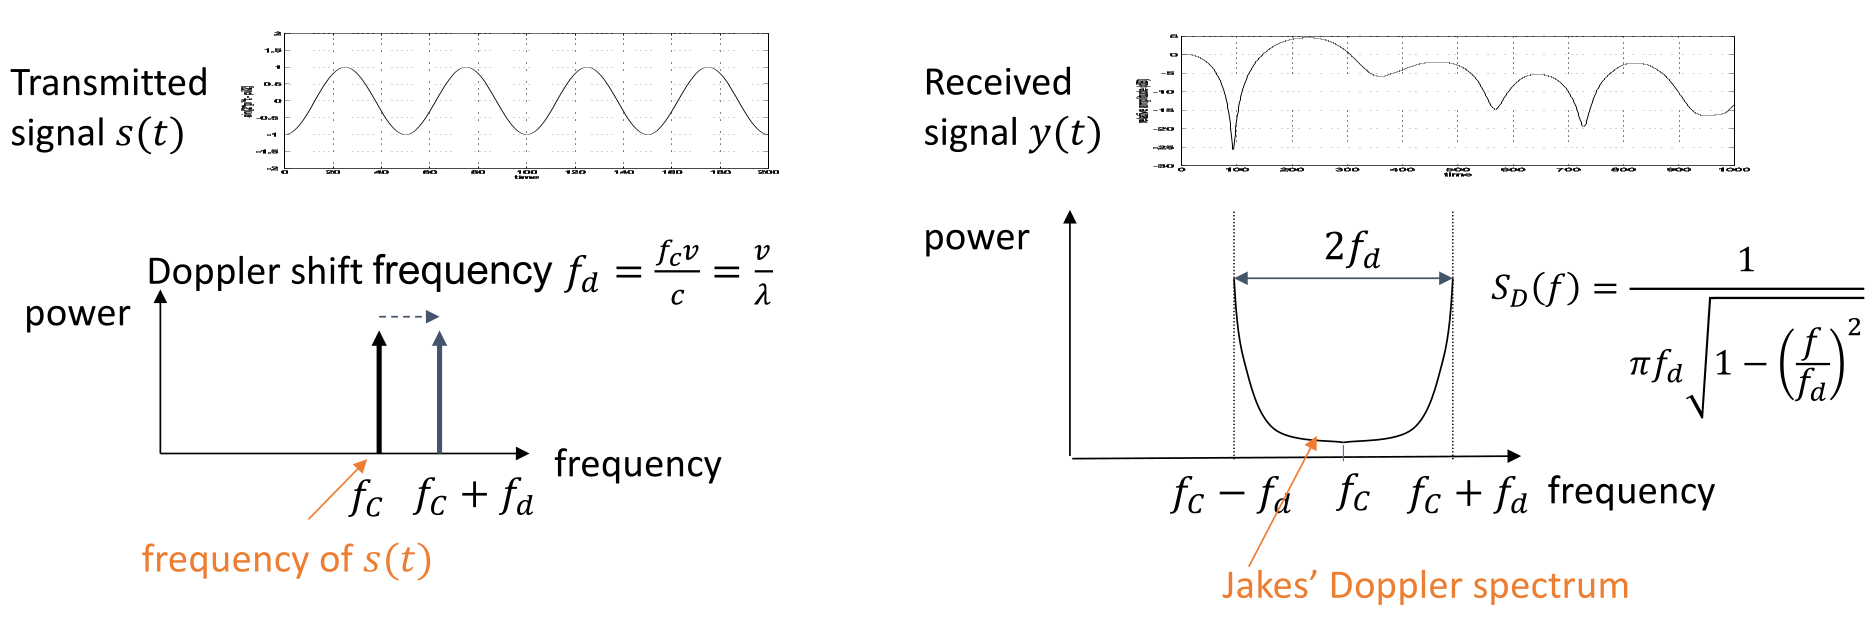
\includegraphics[width=0.875\textwidth]{imgs/jakes.jpg}
    \captionsetup{width=.5\textwidth}
    \caption*{Spettro Doppler di Jakes}
      
\end{figure}


Lo spettro originale è ripetuto su un intervallo maggiore di frequenza. L'effetto prodotto è l'allargamento dello spettro occupato (\textbf{Doppler spread}), derivante dal fatto che il segnale stocastico ricevuto assume la forma:

\[
    y(t) = \alpha(t) s(t)
\]
% TODO da dove deriva la radice quadrata al denominatore considerando v cos(theta) / c
dove $\alpha(t)$ è il guadagno tempo-variante del canale e $s(t)$ è il segnale trasmesso . Quando $f_d$ è trascurabile (e quindi circa 0), $S_D(f)$ diventa circa una delta, e quindi $S_Y(f) = S_S(f)$. In frequenza, la convoluzione tra queste due funzioni produce una funzione la cui durata (tempo) e banda (frequenza) è la somma delle due funzioni di partenza, per questo motivo si ha un un incremento della banda occcupata.

\[
    S_Y(f) = S_S(f) \ast S_D(f)
\]
Supponendo quindi che il segnale inviato fosse $s(t) = \sin(2\pi f_c t)$:
\[
    S_Y(f) = \frac{1}{\pi f_d \sqrt{1 - \left(\frac{f - f_c}{f_d}\right)^2}}
\]
%the result of this is that the spectrum is broadened
Il risultato è che lo spettro del segnale ricevuto è più ampio rispetto a quello trasmesso.
Lo studio della funzione di autocorrelazione del canale wireless nel caso del modello di Jakes permette di giungere alla definizione del \textbf{coherence time}, ovvero l'intervallo temporale entro cui è possibile considerare il canale costante e dunque rappresentabile come un sistema LTI.


\[
    R_D (\tau) = J_0(2\pi f_d \tau) \quad \text{funzione di autocorrelazione time varying channel}
\]

dove $J_0$ è la funzione di Bessel di prima specie di ordine 0.  Se la funzione si annulla il canale può essere considerato non correlato, ovvero il canale nei due istanti assume valori indipendenti e dunque varia.
Per $x=\frac{1}{2}$ si ha che $J_0(2\pi x) = 0$, quindi il canale può considerarsi incorrelato per $\tau = T_c = \frac{1}{2f_d}$.

\[
    f_d T_c = \frac{1}{2} \quad \Rightarrow \quad  T_c = \frac{1}{2 f_d} = \frac{1}{2} \frac{c}{f_c v} \quad \text{coherence time}
\]
Quindi $T_c$ rappresenta il tempo entro cui il canale può essere considerato costante, ovvero un sistema LTI.
\begin{center}
    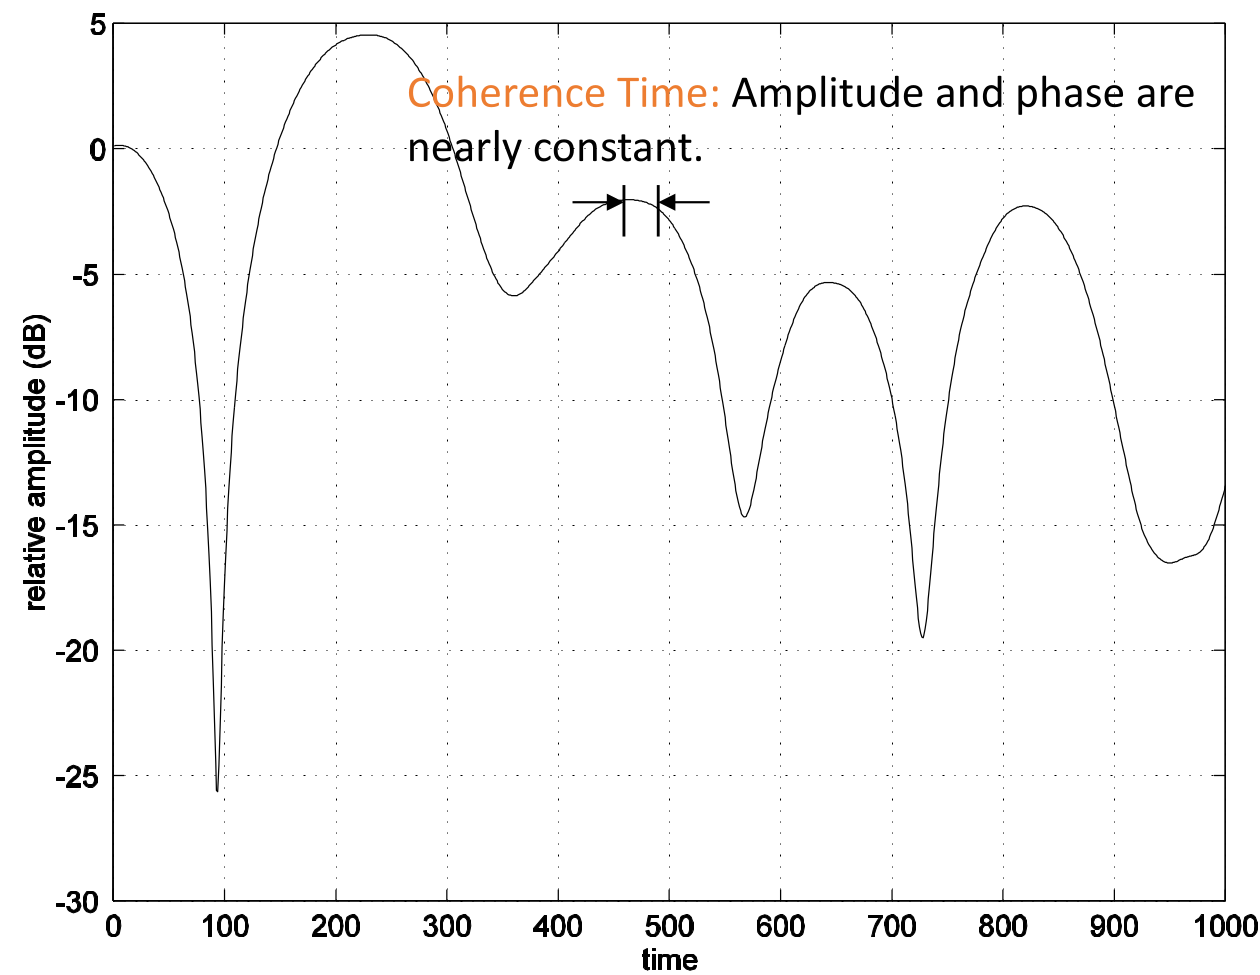
\includegraphics[width=0.5\textwidth]{imgs/coherence_time.png}
\end{center}


Lo stesso concetto può essere espresso anche in termini di distanza, molto importante per l'utilizzo di antenne direzionali.
\[
    d_c = v T_c = \frac{v}{2f_d} = \frac{1}{2} v \frac{c}{f_c v} = \frac{\lambda}{2}
\]
Questo implica che segnali ricevuti a distanze nell'ordine di metà lunghezza d'onda possono essere considerati incorrelati.
Se $T < T_c$ si può asssumere che il canale sia modellabile come LTI in quanto la risposta risulta costante nel tempo per almeno $T_c$, inferiore al tempo dei simboli.
Incrementando il rate si riduce il tempo dei simboli, permettendo di modellare il canale come LTI, tuttavia si rischia di incorrere in un canale frequency selective per cui sono necessarie contromisure per contrastare l'ISI generato.




\begin{center}
    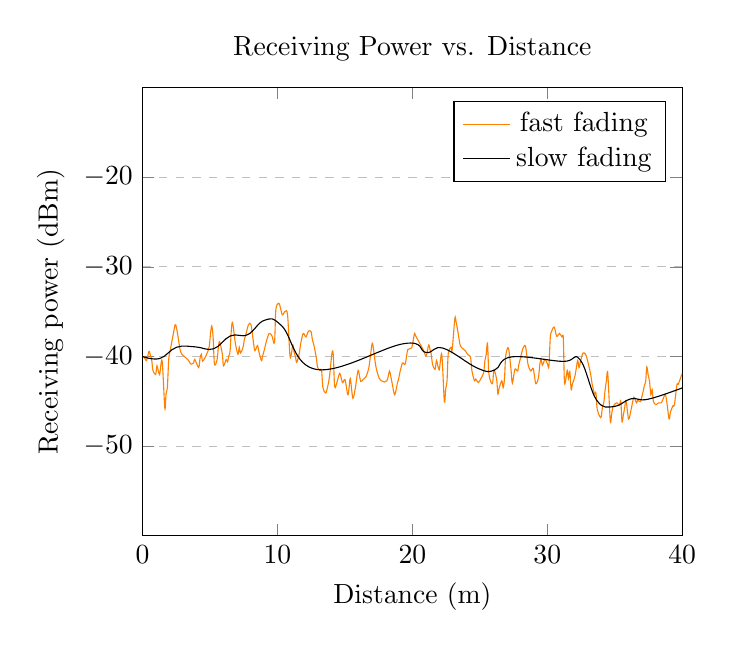
\begin{tikzpicture}
        \begin{axis}[
                title={Receiving Power vs. Distance},
                xlabel={Distance (m)},
                ylabel={Receiving power (dBm)},
                xmin=0, xmax=40,
                ymin=-60, ymax=-10,
                xtick={0,10,20,30,40},
                ytick={-50,-40,-30,-20},
                legend pos=north east,
                ymajorgrids=true,
                grid style=dashed,
            ]

            \addplot[
                color=orange,
                mark=none,
                smooth,
                tension=0.5,
            ]
            coordinates {
                    (0.1,-39.94) (0.29,-40.45) (0.48,-39.42) (0.58,-39.87) (0.68,-40.39) (0.77,-41.55) (0.97,-42.0) (1.07,-41.03) (1.26,-42.0) (1.45,-40.45) (1.65,-45.74) (1.74,-44.19) (1.84,-43.42) (1.94,-40.32) (2.03,-39.48) (2.23,-37.87) (2.42,-36.45) (2.52,-36.84) (2.62,-37.68) (2.81,-39.42) (3.0,-39.87) (3.2,-40.13) (3.39,-40.39) (3.58,-40.84) (3.78,-40.71) (3.87,-40.32) (4.16,-41.23) (4.26,-40.19) (4.36,-39.74) (4.46,-40.52) (4.75,-39.74) (4.94,-38.9) (5.04,-37.42) (5.13,-36.58) (5.23,-37.81) (5.33,-40.84) (5.52,-40.39) (5.62,-38.97) (5.71,-38.32) (5.91,-39.68) (6.0,-41.03) (6.2,-40.32) (6.3,-40.58) (6.39,-39.94) (6.49,-39.35) (6.59,-36.84) (6.68,-36.26) (6.88,-38.52) (7.07,-39.74) (7.17,-38.97) (7.26,-39.61) (7.46,-38.9) (7.55,-38.06) (7.65,-37.61) (7.85,-36.45) (8.04,-36.45) (8.23,-38.52) (8.33,-39.35) (8.52,-38.77) (8.62,-39.42) (8.81,-40.45) (8.91,-39.87) (9.01,-39.35) (9.2,-38.19) (9.39,-37.42) (9.59,-37.68) (9.78,-38.45) (9.88,-34.77) (10.07,-34.06) (10.17,-34.26) (10.36,-35.35) (10.56,-34.97) (10.75,-35.35) (10.94,-40.06) (11.14,-38.71) (11.23,-39.48) (11.33,-40.0) (11.43,-40.65) (11.62,-39.61) (11.72,-38.58) (11.91,-37.42) (12.11,-37.81) (12.3,-37.16) (12.49,-37.23) (12.59,-38.13) (12.69,-38.65) (12.88,-40.13) (12.98,-41.23) (13.17,-41.55) (13.27,-41.48) (13.37,-43.48) (13.56,-44.06) (13.66,-43.74) (13.85,-42.32) (14.04,-39.61) (14.14,-39.81) (14.24,-43.35) (14.43,-42.77) (14.62,-41.87) (14.82,-42.9) (15.01,-42.58) (15.21,-44.26) (15.3,-43.61) (15.4,-42.45) (15.59,-44.65) (15.79,-43.35) (15.98,-41.55) (16.17,-42.77) (16.37,-42.52) (16.56,-42.26) (16.76,-41.35) (16.85,-40.45) (16.95,-39.23) (17.05,-38.52) (17.24,-40.58) (17.34,-41.42) (17.53,-42.39) (17.72,-42.71) (17.92,-42.84) (18.11,-42.71) (18.21,-42.19) (18.31,-41.61) (18.4,-42.19) (18.5,-42.97) (18.69,-44.26) (18.89,-42.97) (18.98,-42.52) (19.08,-41.74) (19.27,-40.71) (19.47,-40.84) (19.66,-39.23) (19.95,-39.03) (20.15,-37.48) (20.24,-37.68) (20.82,-39.29) (21.02,-39.94) (21.21,-38.71) (21.31,-39.23) (21.4,-39.74) (21.5,-40.9) (21.69,-41.42) (21.79,-40.45) (21.99,-41.48) (22.18,-39.74) (22.37,-45.03) (22.47,-43.61) (22.57,-42.71) (22.66,-39.68) (22.86,-38.97) (22.95,-39.29) (23.15,-35.74) (23.24,-36.13) (23.34,-36.9) (23.54,-38.71) (23.73,-39.1) (23.92,-39.35) (24.12,-39.81) (24.31,-40.06) (24.41,-41.55) (24.6,-42.71) (24.7,-42.52) (24.89,-42.9) (25.08,-42.45) (25.28,-41.81) (25.38,-40.45) (25.47,-39.81) (25.57,-38.52) (25.67,-41.87) (25.86,-42.97) (25.96,-42.84) (26.05,-41.48) (26.25,-42.58) (26.34,-44.19) (26.44,-43.48) (26.63,-42.71) (26.73,-43.48) (26.83,-42.45) (26.92,-39.94) (27.12,-39.03) (27.31,-41.42) (27.41,-42.97) (27.6,-41.42) (27.8,-41.61) (27.89,-40.9) (27.99,-40.32) (28.18,-39.16) (28.38,-38.84) (28.57,-40.84) (28.77,-41.61) (28.96,-41.35) (29.15,-43.03) (29.35,-42.32) (29.44,-40.97) (29.54,-40.26) (29.64,-40.97) (29.83,-40.32) (30.02,-40.84) (30.12,-41.1) (30.22,-37.94) (30.31,-37.23) (30.51,-36.71) (30.7,-37.74) (30.9,-37.42) (31.09,-37.81) (31.19,-37.94) (31.28,-42.97) (31.48,-41.55) (31.57,-42.45) (31.67,-41.68) (31.77,-43.68) (31.86,-43.1) (32.06,-42.13) (32.25,-40.45) (32.35,-41.23) (32.45,-40.65) (32.64,-39.61) (32.83,-39.74) (32.93,-40.13) (33.03,-40.71) (33.22,-42.0) (33.32,-43.03) (33.51,-44.19) (33.61,-44.06) (33.7,-45.87) (33.9,-46.71) (34.0,-46.71) (34.09,-45.61) (34.19,-45.16) (34.29,-43.68) (34.38,-42.77) (34.48,-41.81) (34.67,-47.16) (34.77,-46.45) (34.87,-45.61) (35.06,-45.23) (35.16,-45.16) (35.35,-45.42) (35.45,-44.97) (35.54,-47.29) (35.64,-46.52) (35.74,-45.68) (35.84,-44.9) (36.03,-46.97) (36.22,-45.87) (36.42,-44.52) (36.61,-45.16) (36.71,-44.84) (36.9,-45.03) (37.09,-44.0) (37.19,-43.29) (37.29,-42.84) (37.38,-41.16) (37.48,-42.06) (37.58,-42.77) (37.68,-44.26) (37.77,-43.68) (37.87,-45.03) (38.06,-45.35) (38.26,-45.16) (38.45,-45.16) (38.64,-44.52) (38.74,-44.19) (38.84,-44.84) (39.03,-46.97) (39.13,-46.19) (39.32,-45.48) (39.42,-45.42) (39.61,-43.16) (39.71,-43.1) (40.0,-41.94) (40.19,-42.13) (40.39,-41.35) (40.48,-40.13)
                };
            \addlegendentry{fast fading}

            \addplot[
                color=black,
                mark=none,
                smooth,
                tension=0.7,
            ]
            coordinates {
                    (0.0,-40.0) (1.27,-40.22) (2.53,-38.96) (3.92,-38.92) (5.26,-39.14) (6.52,-37.69) (7.79,-37.56) (9.05,-35.95) (10.32,-36.58) (12.94,-41.45) (19.37,-38.56) (21.02,-39.55) (22.29,-39.07) (24.82,-41.29) (26.08,-41.52) (27.35,-40.04) (31.14,-40.54) (32.41,-40.31) (33.67,-44.89) (34.94,-45.58) (36.2,-44.71) (37.47,-44.76) (40, -43.5)
                };

            \addlegendentry{slow fading}

        \end{axis}
    \end{tikzpicture}


\end{center}




\begin{itemize}
    \item \textbf{Slow fading}: l'effetto Doppler è trascurabile ($B_S \gg f_d$, $T_c \gg T$)
    \item \textbf{Fast fading}: l'effetto Doppler distorce notevolmente il segnale, rendendo difficile ridurre il BER ($B_S < f_d, T_c < T$)
\end{itemize}
Dove $T$ è il symbol time, $B_S$ è la banda del segnale, $f_d$ è il Doppler shift, $T_c$ è il tempo di coerenza del canale.
Se la banda del segnale è maggiore del Doppler shift la convoluzione genera un comportamento non molto significativo.

In generale gli effetti LSF determinano la dimensione della cella di copertura, considerando anche la frequenza di trasmissione.


Come esempio, consideriamo il caso di trasmissione di un segnale a una frequenza \( f_c = 2.1 \si{GHz} \) in un'area suburbana. L'utente si muove alla velocità di $90 \si{km/h}$, ovvero \( v = 25 \si{m/s} \). Lo scenario è caratterizzato da un delay spread \( \sigma_\tau = 2 \si{\mu s} \).

Per la trasmissione, la banda del segnale è \( B_s = 2 \si{MHz} \), da cui possiamo approssimare \( T \) come \( T \approx \frac{1}{B_s} = 500 \si{ns} \), rappresentando la durata di un simbolo nella trasmissione dei dati.
Un importante aspetto di questo scenario è il Doppler spread, calcolato utilizzando \( f_d = \frac{f_c v}{c} = \frac{2.1 \times 10 ^9 \si{Hz} \cdot 25 \si{m/s}}{3 \times 10^8 \si{m/s}} = 175\si{Hz}\).
Il tempo di coerenza del canale \( T_c \) è quindi derivato da \( T_c = \frac{1}{2f_d} \approx 3 \si{ms}\), descrivendo il periodo di tempo durante il quale le condizioni del canale sono relativamente costanti.
Inoltre, la banda di coerenza del canale \( B_c \) è calcolata dal delay spread \( \sigma_\tau \), risultando in \( B_c = \frac{1}{5\sigma_\tau} = 100 \si{kHz} \). Questa banda misura l'intervallo di frequenze su cui la risposta del canale rimane uniforme.
Il canale è quindi definibile come \textit{slow} poiché \( B_s \gg f_d \) (ovvero \( T \ll T_c \)), indicando che i cambiamenti nel canale dovuti agli effetti Doppler sono relativamente lenti rispetto alla larghezza di banda del segnale e al tempo di simbolo.
Il canale è anche definibile come \textit{frequency-selective} a causa di \( B_s > B_c \) (ovvero \( T < \sigma_\tau \)), implicando che diversi segmenti della larghezza di banda possono subire variazioni delle caratteristiche di fading.







\begin{center}
    \textbf{Small-Scale Fading} \\
    \textit{(Based on multipath time delay spread)}

    \bigskip

    \begin{tabular}{|c|c|}
        \hline
        \textbf{Flat Fading}           & \textbf{Frequency Selective Fading} \\ \hline
        BW of signal $<$ BW of channel & BW of signal $>$ BW of channel      \\
        Delay spread $<$ Symbol period & Delay spread $>$ Symbol period      \\ \hline
    \end{tabular}
\end{center}



\begin{center}
    \textbf{Small-Scale Fading} \\
    \textit{(Based on Doppler spread)}

    \bigskip

    \begin{tabular}{|c|c|}
        \hline
        \textbf{Fast Fading}                                      & \textbf{Slow Fading}                                      \\ \hline
        High Doppler spread                                       & Low Doppler spread                                        \\
        Coherence time $<$ Symbol period                          & Coherence time $>$ Symbol period                          \\
        Channel variations faster than baseband signal variations & Channel variations slower than baseband signal variations \\ \hline
    \end{tabular}
\end{center}

\bigskip

\begin{center}
    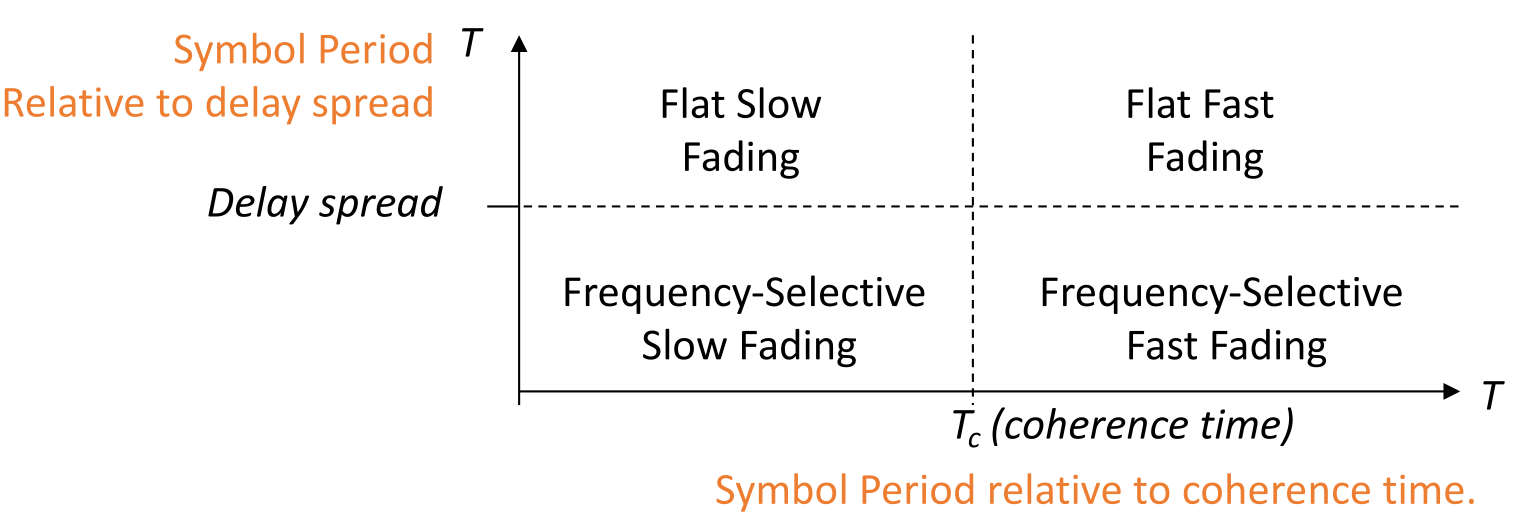
\includegraphics[width=0.75\textwidth]{imgs/recap_ssf1.png}
\end{center}
\begin{center}
    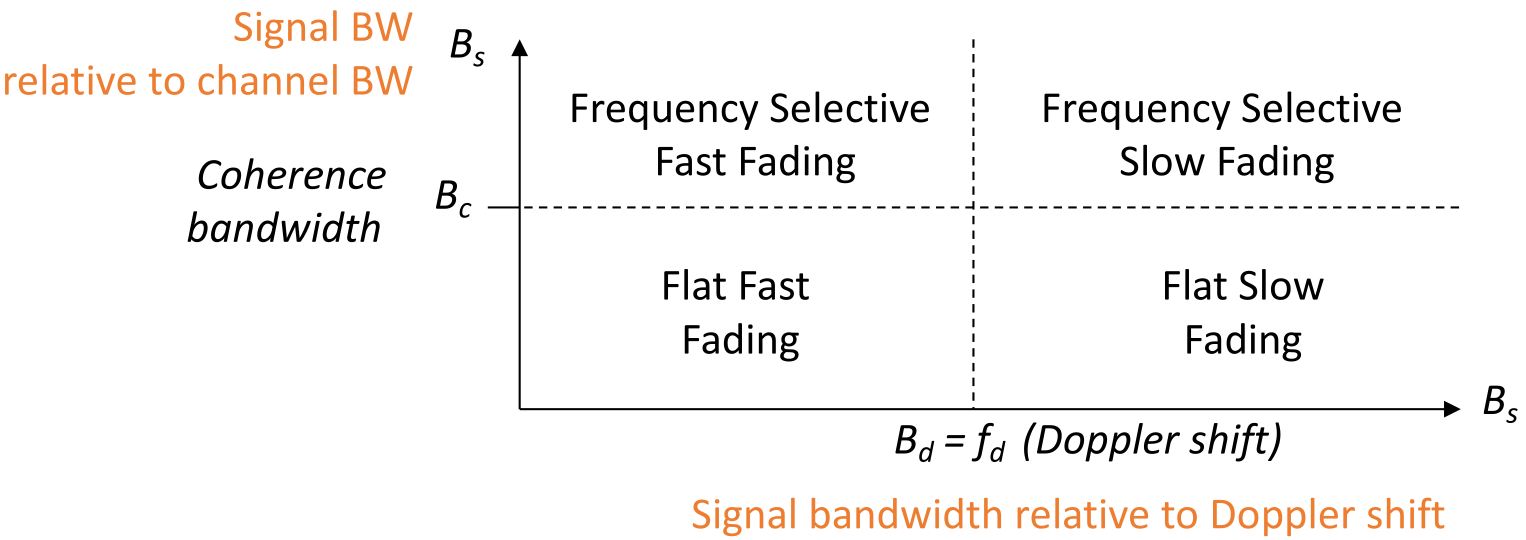
\includegraphics[width=0.75\textwidth]{imgs/recap_ssf2.png}
\end{center}